\documentclass{standalone}
\usepackage{tikz}
\usepackage{ctex,siunitx}
\usepackage{tkz-euclide}
\usepackage{amsmath}
\usetikzlibrary{patterns, calc}
\usetikzlibrary {decorations.pathmorphing, decorations.pathreplacing, decorations.shapes,}
\begin{document}
\small
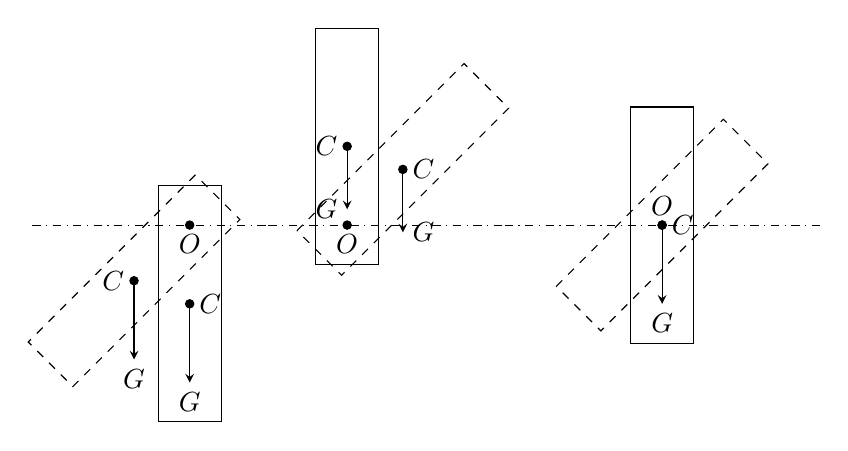
\begin{tikzpicture}[>=stealth,scale=1.0]
  \begin{scope}
    \draw[dashdotted] (-2,0)--(1,0);
    \draw (-.4,.5) rectangle (.4, -2.5);
    \draw[rotate=-45, dashed] (-.4,.5) rectangle (.4, -2.5);
    \draw [fill=black](0,0)  circle (1.5pt) node [below]{$O$};
    \draw [fill=black](0,-1)  circle (1.5pt) node [right]{$C$};
    \draw [fill=black](-135:1)  circle (1.5pt) node [left]{$C$};
    \draw[->] (0,-1)--(0,-2)node [below]{$G$};
    \draw[->] (-135:1)--+(0,-1)node [below]{$G$};
  \end{scope}
  \begin{scope}[xshift=2cm]
    \draw[dashdotted] (-1,0)--(2,0);
    \draw (-.4,-.5) rectangle (.4, 2.5);
    \draw[rotate=-45, dashed] (-.4,-.5) rectangle (.4, 2.5);
    \draw [fill=black](0,0)  circle (1.5pt) node [below]{$O$};
    \draw [fill=black](0,1)  circle (1.5pt) node [left]{$C$};
    \draw [fill=black](45:1)  circle (1.5pt) node [right]{$C$};
    \draw[->] (0,1)--(0,.2)node [left]{$G$};
    \draw[->] (45:1)--+(0,-.8)node [right]{$G$};
  \end{scope}
  \begin{scope}[xshift=6cm]
    \draw[dashdotted] (-2,0)--(2,0);
    \draw (-.4,-1.5) rectangle (.4, 1.5);
    \draw[rotate=-45, dashed] (-.4,-1.5) rectangle (.4, 1.5);
    \draw [fill=black](0,0)  circle (1.5pt) node [above]{$O$};
    \draw [fill=black](0,0)  circle (1.5pt) node [right]{$C$};
    \draw[->]  (0,0)--(0,-1)   node [below]{$G$};
  \end{scope}
\end{tikzpicture}
\end{document}